% rubber: set program xelatex
\documentclass{beamer}
\usetheme[faculty=fi,logoPath=/home/jptiz/dev/edu/gba-nds-classes/gba/0_intro/slides/,logo=logo-pet-1]{fibeamer}
\usepackage[main=portuguese,english]{babel}
\selectlanguage{portuguese}
\usepackage{fontspec}

\usepackage{booktabs}
\usepackage{csquotes}
\usepackage{colortbl}
\usepackage{graphicx}
\usepackage{minted}
\usepackage{multicol}
\usepackage{tikz}

\graphicspath{{img/}}

\let\emph\relax % there's no \RedeclareTextFontCommand
\DeclareTextFontCommand{\emph}{\bfseries\em}

\newcolumntype{C}{>{\columncolor[rgb]{.9,.6,.6}}c}
\newcolumntype{A}{>{\columncolor{cyan}}c}
\newcolumntype{R}{>{\columncolor{red}}c}
\newcolumntype{G}{>{\columncolor[rgb]{0,.5,0}}c}
\newcolumntype{B}{>{\columncolor{blue}}c}
\newcolumntype{K}{>{\columncolor{black}}c}

\title{Curso de Desenvolvimento GBA}
\subtitle{1. Introdução ao GBA}
\author{João Paulo Taylor Ienczak Zanette}

\begin{document}

\maketitle

\begin{darkframes}
\begin{frame}[allowframebreaks]{Índice}
    \tableofcontents
\end{frame}

\section{Introdução}
\subsection{Contextualização do Curso}

\begin{frame}{Objetivos}
    \begin{itemize}
        \item Ensinar programação de baixo-nível (comunicação direta com
            hardware/integração com assembly);
        \item Ensinar técnicas de programação aplicadas;
        \item Mostrar o funcionamento de imagens/gráficos e áudio no mundo
            digital;
        \item Relacionar as tecnologias vistas com as utilizadas
            atualmente.
    \end{itemize}
\end{frame}

\begin{frame}{Programação}
    \begin{itemize}
        \item Assembly ARM7-TDMI --- Modo Thumb (GBA);
        \item OpenGL (NDS);
        \item C++ (GBA/NDS).
    \end{itemize}

    A mesma forma de programação para GBA serve também para: GB, GBC, NES,
    SNES, MegaDrive, SegaSaturn e PSX (PS1).
\end{frame}

\begin{frame}{Circuitos e Técnicas Digitais}
    \begin{itemize}
        \item Leitura/escrita de registradores (em que cada bit é mapeado
            para uma função específica) via programação;
    \end{itemize}
\end{frame}

\begin{frame}{Sistemas Digitais}
    \begin{itemize}
        \item Compreensão a respeito de como o Assembly gerado pela
            compilação altera o estado/memória do circuito;
        \item Compreensão do sistema que gera imagens em um circuito
            digital (VGA, LCD, etc\ldots);
        \item Funcionamento (inclusive a nível de circuito) da execução de
            músicas em formato de instrução MIDI\@;
        \item Técnicas de otimização através de Hardware.
    \end{itemize}
\end{frame}

\begin{frame}{Computação Gráfica}
    \begin{itemize}
        \item Desenho de primitivas (linhas, triângulos, círculos, etc\ldots);
        \item Aceleração gráfica via Hardware.
    \end{itemize}
\end{frame}

\begin{frame}{Notações}
    \begin{center}
        \begin{tabular}{r|l}
            \texttt{0b???}      & \enquote{???} está em binário (\texttt{0b11111111 = 255}).\\
            \texttt{0x???}      & \enquote{???} está em hexadecimal (\texttt{0xFF = 255}).\\
            \texttt{???b}       & \enquote{???} está em binário (\texttt{11111111b = 255}).\\
            \texttt{???h}       & \enquote{???} está em hexadecimal (\texttt{FFh = 255}).\\
            \texttt{????:????}  & \enquote{:} serve apenas para melhor visualização \\
                                & (\texttt{0x04000000 = 0400:0000h}).\\
            \texttt{??? $>>$ x} & \enquote{???} deslocado ``x''\ bits para direita.\\
            \texttt{??? $<<$ x} & \enquote{???} deslocado ``x''\ bits para esquerda.\\
        \end{tabular}
    \end{center}
\end{frame}


\subsection{Evolução dos consoles}
\begin{frame}{\huge Hello, World!}
    \begin{multicols}{2}
        Um breve prólogo das especificações técnicas e limitações dos consoles de
        VideoGame ao longo do tempo e uma análise de sua evolução.
        \begin{figure}[h!]
            \centering
            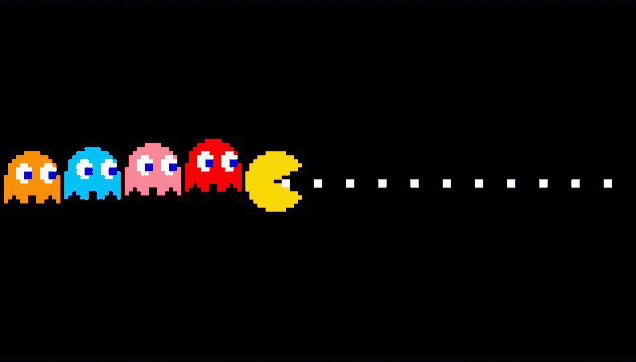
\includegraphics[width=.5\textwidth]{pacman}
        \end{figure}
    \end{multicols}
\end{frame}

\begin{frame}{Atari 2600 (1977)}
    \begin{multicols}{2}
        \begin{description}
            \item[Processador:] MOS Technology 6507 (variante do 6502 de 1975)
            \item[Barramento:] 8 bits
            \item[Clock:] 1.19MHz
            \item[RAM:] 128 bytes
            \item[ROM:] 16KB
            \item[Resolução:]
                \begin{itemize}
                    \item 160$\times$192 (NTSC)
                    \item 160$\times$228 (PAL)
                \end{itemize}
            \item[Cores:] 128
            \item[Som:] 2 canais (1 chip cada)
        \end{description}
    \end{multicols}
    \begin{figure}[h!]
        \centering
        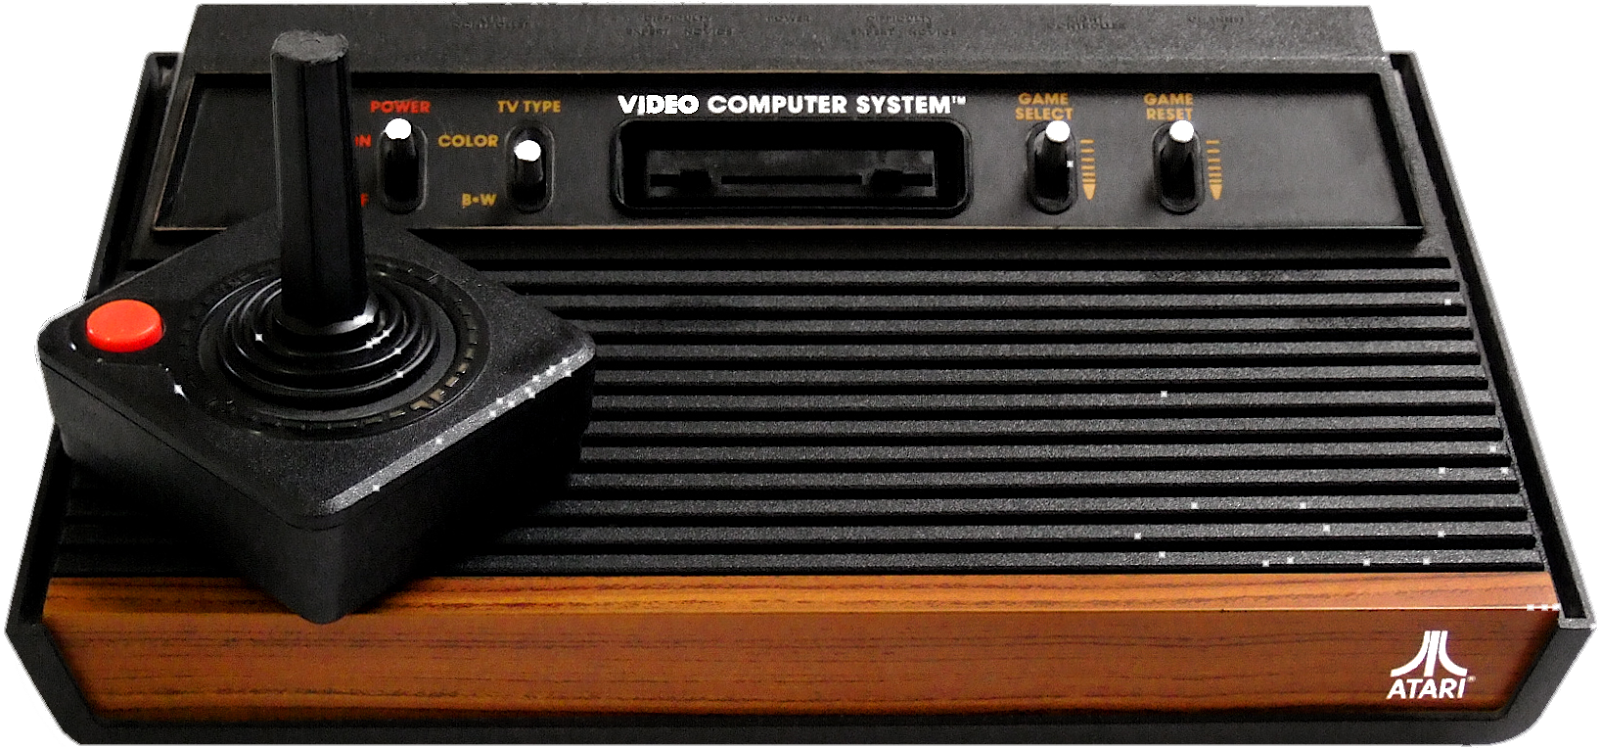
\includegraphics[width=.5\textwidth]{Atari2600}
    \end{figure}
\end{frame}

\begin{frame}{NES (1983)}
    \begin{multicols}{2}
        \scriptsize
        \begin{description}
            \setlength\itemsep{0em}
            \item[Processador:] MOS 6502 Customizado
            \item[Barramento:] 8 bits
            \item[Clock (CPU):] 1.79MHz (NTSC), 1.66MHz (PAL)
            \item[Clock (GPU):] 5.37MHz (NTSC), 5.33MHz (PAL)
            \item[RAM:] 2KiB + RAM Expandida (do cartucho)
            \item[ROM:] 48KB
            \item[Resolução:] 256$\times$240
            \item[Cores:] 56 cores (paleta básica)
            \item[Cores na tela:] 25 cores por scanline (cor de fundo + 4
                conjuntos de 3 cores de tiles + 4 conjuntos de cores por
                sprite)
            \item[OAM:] 256 bytes
            \item[Dim.\ das Sprites:] 16$\times$16 ou 24$\times$24
            \item[Máx. Sprites na tela:] 64
            \item[Som:] 5 canais (2 square, 1 triangle, 1 ruído-branco, 1
                modulação de código delta-pulse (DPCM) de 6 bits)
        \end{description}
    \end{multicols}
    \begin{multicols}{2}
        \begin{figure}[h!]
            \centering
            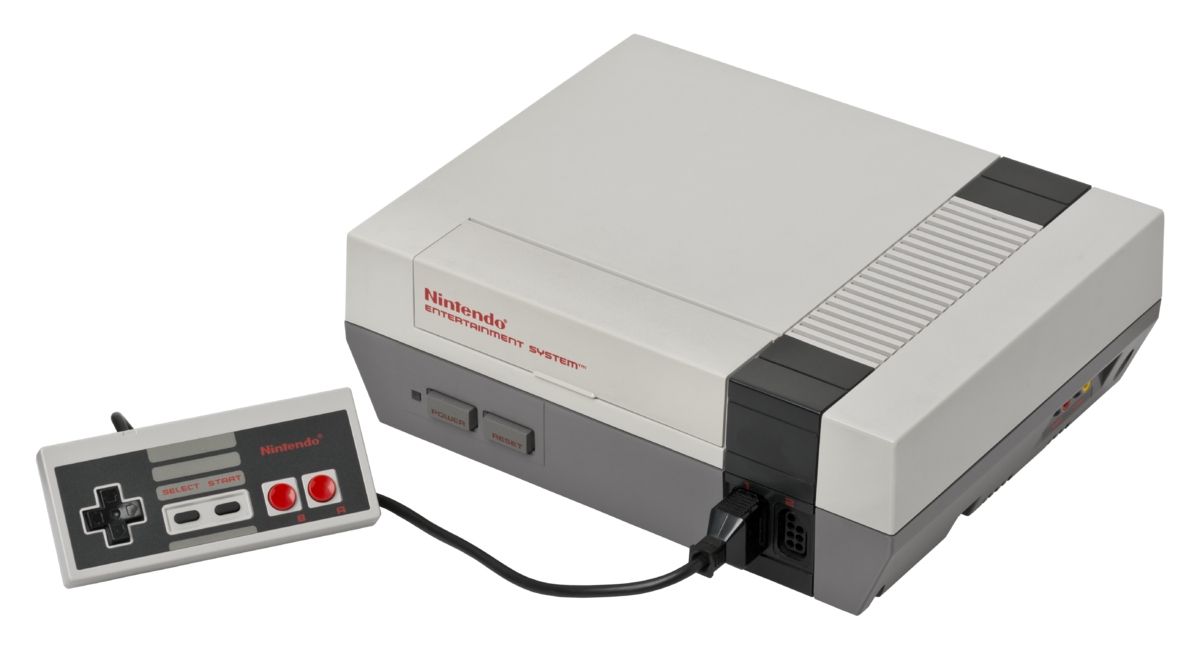
\includegraphics[height=.2\textheight]{nes}
        \end{figure}
        \begin{figure}[h!]
            \centering
            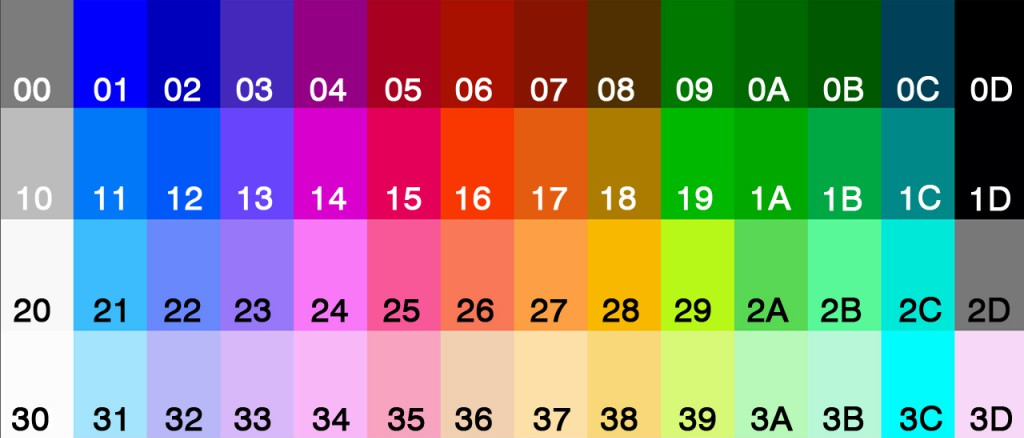
\includegraphics[height=.2\textheight]{nes_palette}
        \end{figure}
    \end{multicols}
\end{frame}

\begin{frame}{SNES (1990)}
    \begin{multicols}{2}
        \scriptsize
        \begin{description}
            \setlength\itemsep{0em}
            \item[Processador:] Ricoh 5A22 customizado da Nintendo
            \item[Barramento:] 16 bits
            \item[Clock (CPU):] 1.79MHz, 2.86MHz ou 3.58MHz
            \item[Clock (GPU):] Mesmo da CPU
            \item[RAM:] 128KB
            \item[VRAM:] 64KB (512 + 32 bytes de sprite, 256$\times$15 bits de
                paleta)
            \item[RAM (Áudio):] 64KB
            \item[Resolução:] 256$\times$224/512$\times$448
            \item[Cores:] 32768 (15 bits)
            \item[OAM:] 544 bytes
            \item[Dim.\ das sprites:] 8$\times$8, 16$\times$16, 32$\times$32 e 64$\times$64
            \item[Cores/sprite:] 16
            \item[Máx.\ sprites na tela:] 128 (32 na mesma linha)
            \item[Camadas de background:] 4
            \item[Som:] 8 canais (32KHz 16-bit stereo).
        \end{description}
    \end{multicols}
    \begin{multicols}{2}
        \begin{figure}[h!]
            \centering
            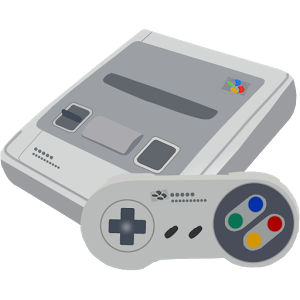
\includegraphics[height=.2\textheight]{snes}
        \end{figure}
        \begin{figure}[h!]
            \centering
            
\includegraphics[height=.2\textheight]{snes_palette}
        \end{figure}
    \end{multicols}
\end{frame}

\begin{frame}{GameBoy (1989)}
    \begin{multicols}{2}
        \scriptsize
        \begin{description}
            \setlength\itemsep{0em}
            \item[Processador:] Sharp LR35902 Customizado
            \item[Barramento:] 8 bits
            \item[Clock (CPU):] 4.19MHz
            \item[RAM:] 8KB (podendo ser expandido para 32KB)
            \item[ROM:] 256 bytes (interno),
                256K/512K/1M/2M/4M/8M (cartuchos)
            \item[VRAM:] 8KB (interno)
            \item[Resolução:] 160x144
            \item[Cores:] 2 bits (4 tons de \enquote{cinza})
            \item[OAM:] 160 bytes (4 bytes/sprite)
            \item[Dim.\ das sprites:] 8x8, 8x16
            \item[Cores/sprite:] 16
            \item[Máx.\ sprites na tela:] 40
            \item[Som:] 2 geradores de pulso de onda
        \end{description}
    \end{multicols}
    \begin{multicols}{2}
        \begin{figure}[h!]
            \centering
            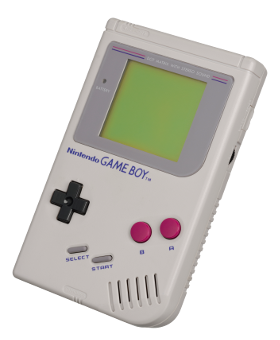
\includegraphics[height=.2\textheight]{gb}
        \end{figure}
        \begin{figure}[h!]
            \centering
            
\includegraphics[height=.2\textheight]{gb_palette}
        \end{figure}
    \end{multicols}
\end{frame}

\begin{frame}{GameBoy Advance (2001)}
    \vspace{-1em}
    \begin{multicols}{2}
        \scriptsize
        \begin{description}
            \setlength\itemsep{0em}
            \item[Processador:] ARM7-TDMI com memória embarcada
            \item[Barramento:] 16 bits
            \item[Co-processador:] Z80 8-bit de 4/8MHz (para
                compatibilidade com GB/GBC)
            \item[Clock (CPU/GPU):] 16.8MHz/\textasciitilde5.5MHz (\textbf{59.73FPS})
            \item[SRAM/DRAM:] 32KB/256KB
            \item[VRAM:] 92KB (interno)
            \item[Resolução:] 240x160 (3:2)
            \item[Cores:] 15-bit BGR (5 bits/canal), 512 cores (character
                mode), 32768 cores (bitmap mode)
            \item[OAM:] 1KB (128 objetos de 3x16bit, 32 transformações de objetos de 4x16bit)
            \item[Dim.\ das sprites:] 8x8, 8x16, 8x32, 16x8, 16x16, 16x32,
                32x8, 32x16, 32x32, 32x64, 64x32, 64x64
            \item[Máx.\ sprites na tela:] 256
            \item[Som:] Dual 8-bit DAC para som Stereo (DirectSound)
        \end{description}
    \end{multicols}
    \begin{multicols}{2}
        \begin{figure}[h!]
            \centering
            
\includegraphics[height=.2\textheight]{gba}
        \end{figure}
        \begin{figure}[h!]
            \centering
            
\includegraphics[height=.2\textheight]{snes_palette}
        \end{figure}
    \end{multicols}
\end{frame}

\begin{frame}{GameBoy Advance (2001)}
    \begin{description}
        \item[ARM7-TDMI]: ARM7 + 16-bit \underline{T}humb + JTAG
            \underline{D}ebug + fast \underline{M}ultiplier + enhanced
            \underline{I}CE.
        \item[DAC:]
            \underline{D}igital-\underline{A}nalogic-\underline{C}onverter
    \end{description}
\end{frame}

\section{Conhecendo a plataforma}
\subsection{O interior do GBA}
\begin{frame}{}
    \huge \textbf{O interior do GBA}
\end{frame}

\begin{frame}{Interior do GBA (frontal)}
    \begin{figure}[h!]
        \centering
        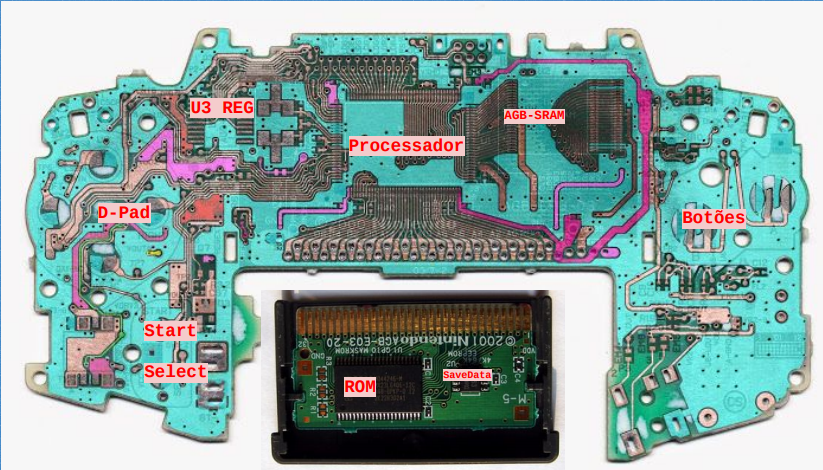
\includegraphics[width=1\textwidth,height=1\textheight,keepaspectratio]{gba_inside_front}
    \end{figure}
\end{frame}

\begin{frame}{Interior do GBA (frontal)}
    \begin{figure}[h!]
        \centering
        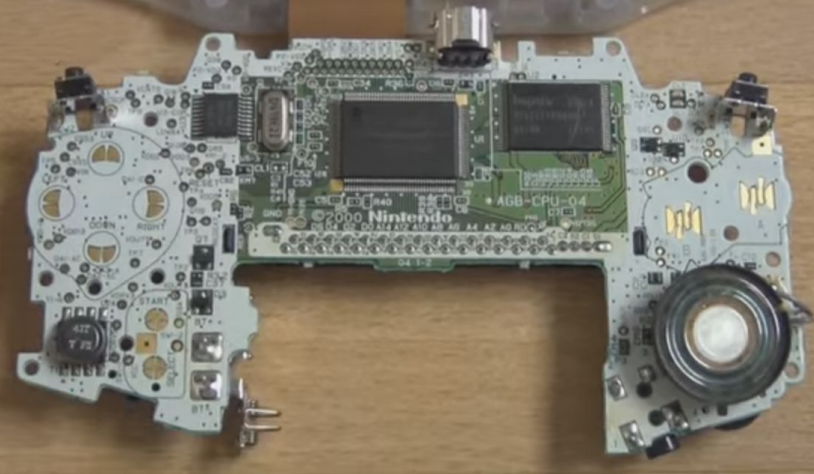
\includegraphics[width=1\textwidth,height=1\textheight,keepaspectratio]{gba_inside_front_real}
    \end{figure}
\end{frame}

\begin{frame}{Interior do GBA (trás)}
    \begin{figure}[h!]
        \centering
        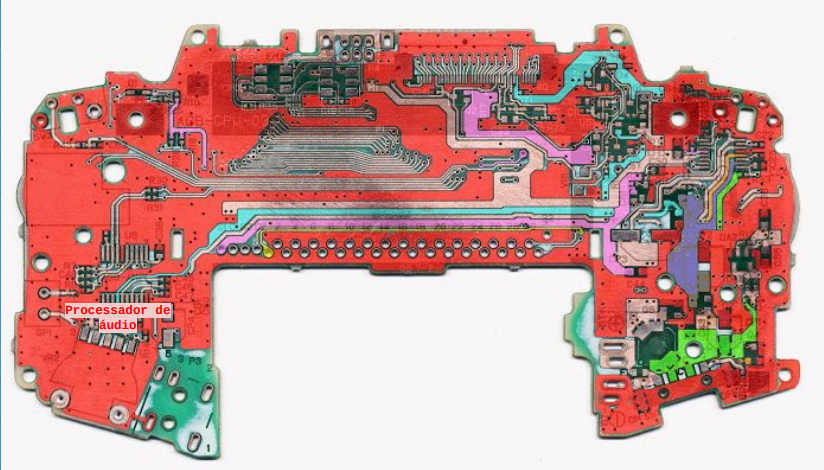
\includegraphics[width=1\textwidth,height=1\textheight,keepaspectratio]{gba_inside_back}
    \end{figure}
\end{frame}

\begin{frame}{Interior do GBA: Processador}
    \begin{figure}[h!]
        \centering
        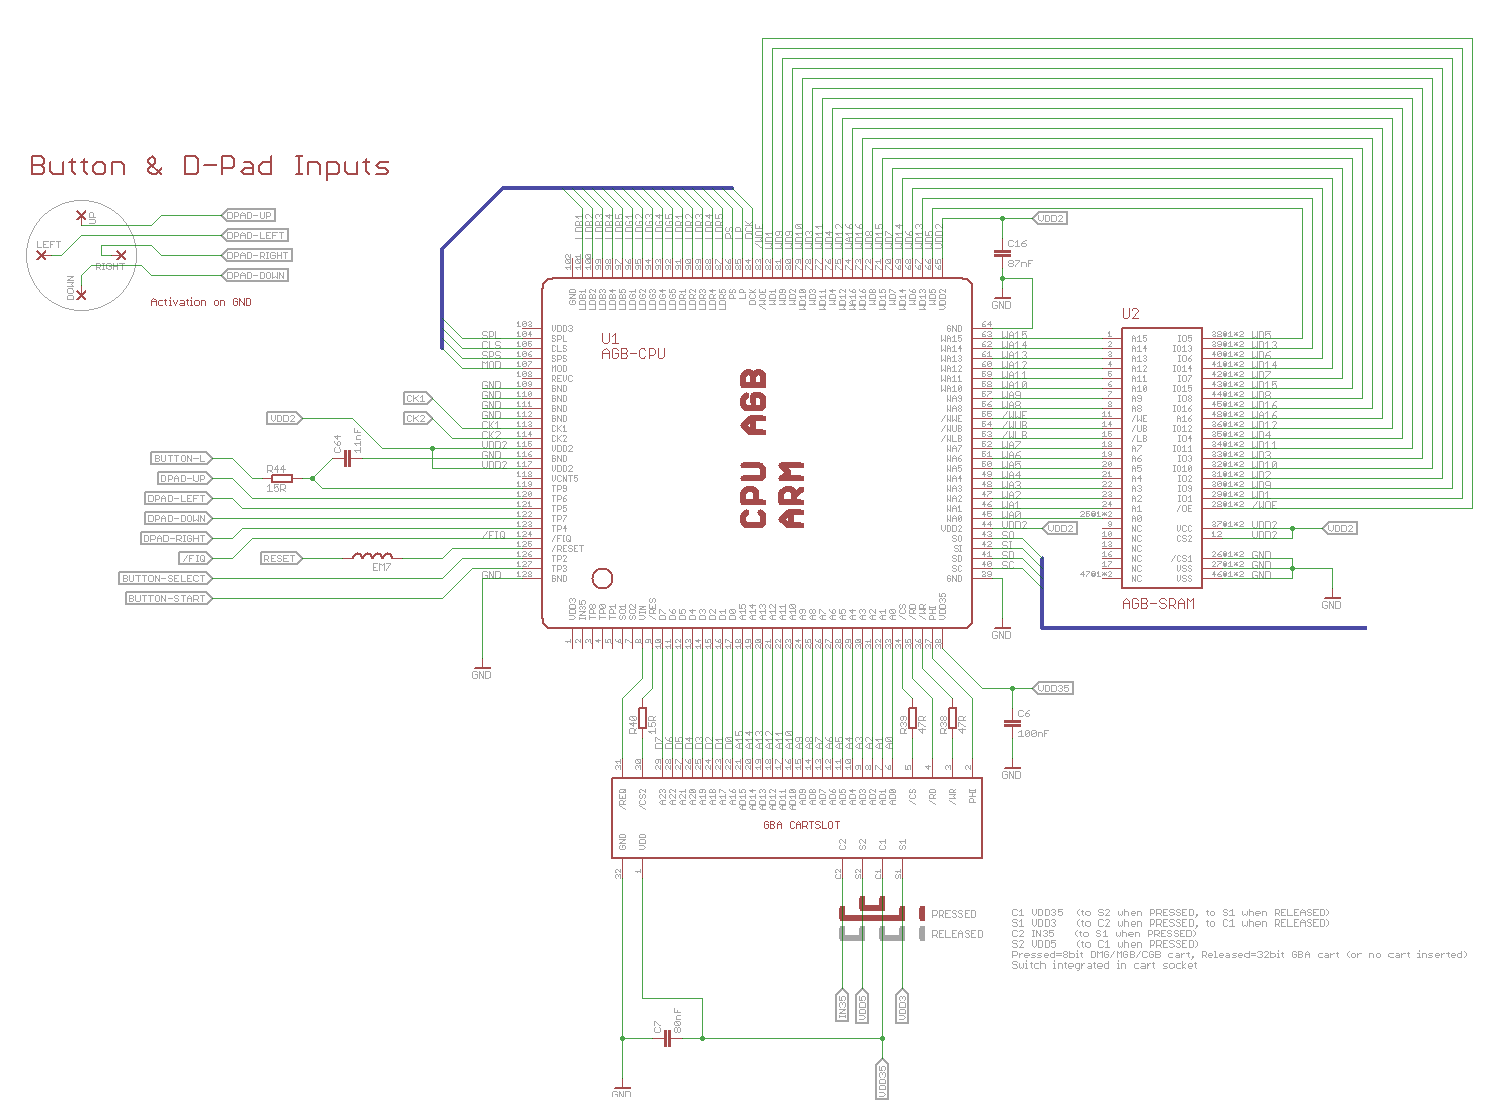
\includegraphics[width=0.95\textwidth,height=0.95\textheight,keepaspectratio]{gba_processor}
    \end{figure}
\end{frame}

\begin{frame}{Organização da Memória (Geral)}
    \begin{center}
        \begin{tabular}{|r|c|l|}
            \hline
            Descrição              & Início               & Tamanho \\\hline
            BIOS -- ROM do Sistema & \texttt{0x00XX:XXXX} & \texttt{0x0:3FFF (16KB)} \\\hline
            WorkRAM On-Board       & \texttt{0x02XX:XXXX} & \texttt{0x3:FFFF (256KB)} \\\hline
            WorkRAM On-Chip        & \texttt{0x03XX:XXXX} & \texttt{0x0:7FFF (32KB)} \\\hline
            Registradores de I/O   & \texttt{0x04XX:XXXX} & \texttt{0x0:03FE (\textasciitilde1KB)} \\\hline
        \end{tabular}
    \end{center}
\end{frame}

\begin{frame}{Organização da Memória (Vídeo)}
    \begin{center}
        \begin{tabular}{|r|c|l|}
            \hline
            Descrição             & Início               & Tamanho \\\hline
            Paleta de BG/OBJ      & \texttt{0x05XX:XXXX} & \texttt{0x0:03FF (1KB)} \\\hline
            RAM de Vídeo (VRAM)   & \texttt{0x06XX:XXXX} & \texttt{0x1:7FFF (96KB)} \\\hline
            OAM (Obj. Attr. Mem.) & \texttt{0x07XX:XXXX} & \texttt{0x0:03FF (1KB)} \\\hline
        \end{tabular}
    \end{center}
\end{frame}

\begin{frame}{Organização da Memória (GamePak)}
    \begin{center}
        \begin{tabular}{|r|c|l|}
            \hline
            Descrição      & Início               & Tamanho \\\hline
            FlashROM (ws0) & \texttt{0x08XX:XXXX} & \texttt{0x1FF:FFFF (16KB)} \\\hline
            FlashROM (ws1) & \texttt{0x0AXX:XXXX} & \texttt{0x1FF:FFFF (256KB)} \\\hline
            FlashROM (ws2) & \texttt{0x0CXX:XXXX} & \texttt{0x1FF:FFFF (32KB)} \\\hline
            GamePakSRAM    & \texttt{0x0EXX:XXXX} & \texttt{0xFFF:FFFF (64KB)} \\\hline
        \end{tabular}
    \end{center}
\end{frame}

\section{Vídeo}
\subsection{Funcionamento}

\begin{frame}{}
    \huge \textbf{\secname}
\end{frame}

\begin{frame}{\secname: \subsecname}
    Vimos que o GBA possui uma tela com resolução 240x160 pixels. Porém,
    isso varia do \emph{modo de vídeo} (Video Mode).

    No GBA há 3 modos \emph{Bitmapeados} (enumerados como 3, 4 e 5) e 3
    modos \emph{Tilemapeados} (enumerados como 0, 1 e 2). Por simplicidade,
    começaremos com modos Bitmapeados (especificamente o 3).

    \begin{center}
        \begin{tabular}{|c|c|c|c|c|c|c|}
            \hline
            Modo & BGs & Resolução        & bpp & RAM                    & Page-Flip \\\hline
            3    & 2   & \texttt{240x160} & 16  & \texttt{(1x)\ 12C00h}  & Não       \\\hline
            4    & 2   & \texttt{240x160} & 8   & \texttt{(2x)\ \ 9600h} & Sim       \\\hline
            5    & 2   & \texttt{160x128} & 16  & \texttt{(2x)\ \ A000h} & Sim       \\\hline
        \end{tabular}
    \end{center}
\end{frame}

\subsection{Registrador de Controle do Visor}
\begin{frame}{\secname: \subsecname}
    \scriptsize\texttt{\begin{center}
        \begin{tabular}{|c|c|c|c|c|c|c|c|c|c|c|c|c|c|c|c|}
            \hline
            F & E & D & C & B & A & 9 & 8 & 7 & 6 & 5 & 4 & 3 & 2 & 1 & 0 \\\hline
            W & W & W & OB & B3 & B2 & B1 & B0 & F & O & H & P & C & \multicolumn{3}{|c|}{Mode} \\\hline
        \end{tabular}
    \end{center}}

    \scriptsize{\begin{center}
        \begin{tabular}{|l|l|}
            \hline
            Bit & \multicolumn{1}{|c|}{Descrição} \\\hline
            \texttt{M (0-2)} & Display-Mode. \\\hline
            \texttt{C (3)} & (Read-Only) Indica se o cartucho inserido é de GBC (1) ou GBA (0). \\\hline
            \texttt{P (4)} & Seleção de página. \\\hline
            \texttt{H (5)} & Habilita acesso à OAM quando em HBlank. \\\hline
            \texttt{O (6)} & Modo de mapeamento de objetos.\\
                           & 0 = 2D/Matricial; 1 = 1D/Sequencial. \\\hline
            \texttt{F (7)} & Força uma tela em branco. \\\hline
            \texttt{B<X> (8-B)} & Habilita Background <X>. \\\hline
            \texttt{OB (C)} & Habilita camada de objetos. \\\hline
            \texttt{W (D-F)} & Habilita o uso das janelas 0/1/de objetos, respectivamente. \\
                             & Janelas podem ser usadas como máscaras (como foi feito com o \\
                             & lampião em Zelda). \\\hline
        \end{tabular}
    \end{center}}
\end{frame}

\begin{frame}{\secname: \subsecname}
    \scriptsize\texttt{\begin{center}
        \begin{tabular}{|c|c|c|c|A|A|A|A|c|c|c|c|c|C|C|C|}
            \hline
            F & E & D & C  & B  & A  & 9  & 8  & 7 & 6 & 5 & 4 & 3 & 2 & 1 & 0 \\\hline
            W & W & W & OB & B3 & B2 & B1 & B0 & F & O & H & P & C & \multicolumn{3}{|C|}{Mode} \\\hline
        \end{tabular}
    \end{center}}

    \scriptsize{\begin{center}
        \begin{tabular}{|l|l|}
            \hline
            Bit & \multicolumn{1}{|c|}{Descrição} \\\hline
            \rowcolor[rgb]{.9,.6,.6}\texttt{M (0-2)} & Display-Mode. \\\hline
            \texttt{C (3)} & (Read-Only) Indica se o cartucho inserido é de GBC (1) ou GBA (0). \\\hline
            \texttt{P (4)} & Seleção de página. \\\hline
            \texttt{H (5)} & Habilita acesso à OAM quando em HBlank. \\\hline
            \texttt{O (6)} & Modo de mapeamento de objetos.\\
                           & 0 = 2D/Matricial; 1 = 1D/Sequencial. \\\hline
            \texttt{F (7)} & Força uma tela em branco. \\\hline
            \rowcolor{cyan}\texttt{B<X> (8-B)} & Habilita Background <X>. \\\hline
            \texttt{OB (C)} & Habilita camada de objetos. \\\hline
            \texttt{W (D-F)} & Habilita o uso das janelas 0/1/de objetos, respectivamente. \\
                             & Janelas podem ser usadas como máscaras (como foi feito com o \\
                             & lampião em Zelda). \\\hline
        \end{tabular}
    \end{center}}
\end{frame}

\begin{frame}{\secname: \subsecname}
    O \emph{Mode 3} usa o BG2 para renderizar, então precisamos habilitar o bit do Mode 3.
    É necessário também habilitar o próprio \emph{Mode 3} em si. Para isso,
    o campo representado pelos \textit{bits} 0, 1 e 2 precisa conter o valor "3",
    que em binário é representado por \texttt{0b11}.

    \scriptsize\texttt{\begin{center}
        \begin{tabular}{|c|c|c|c|c|c|c|c|c|c|c|c|c|c|c|c|}
            \hline
            \ldots & B  & \cellcolor{cyan}A  & 9  & 8  & 7 & 6 & 5 & 4 & 3 & \cellcolor[rgb]{.9,.6,.6}2 & \cellcolor[rgb]{.9,.6,.6}1 & \cellcolor[rgb]{.9,.6,.6}0 \\\hline
            \ldots & B3 & \cellcolor{cyan}B2 & B1 & B0 & F & O & H & P & C & \multicolumn{3}{|C|}{Mode} \\\hline
            \ldots & 0  & \color{red}1  & 0  & 0  & 0 & 0 & 0 & 0 & 0 & 0 & \color{red}1 & \color{red}1 \\\hline
            \ldots & $2^{11}$ & \color{red}$2^{10}$ & $2^9$ & $2^8$ & $2^7$ & $2^6$ & $2^5$ & $2^4$ & $2^3$ & $2^2$ & \color{red}$2^1$ & \color{red}$2^0$ \\\hline
        \end{tabular}
    \end{center}}
\end{frame}

\begin{frame}[fragile]{\secname: \subsecname}
    \vspace{-1em}
    \scriptsize\texttt{\begin{center}
        \begin{tabular}{|c|c|c|c|c|c|c|c|c|c|c|c|c|c|c|c|}
            \hline
            \ldots & B  & \cellcolor{cyan}A  & 9  & 8  & 7 & 6 & 5 & 4 & 3 & \cellcolor[rgb]{.9,.6,.6}2 & \cellcolor[rgb]{.9,.6,.6}1 & \cellcolor[rgb]{.9,.6,.6}0 \\\hline
            \ldots & B3 & \cellcolor{cyan}B2 & B1 & B0 & F & O & H & P & C & \multicolumn{3}{|C|}{Mode} \\\hline
            \ldots & 0  & \color{red}1  & 0  & 0  & 0 & 0 & 0 & 0 & 0 & 0 & \color{red}1 & \color{red}1 \\\hline
            \ldots & $2^{11}$ & \color{red}$2^{10}$ & $2^9$ & $2^8$ & $2^7$ & $2^6$ & $2^5$ & $2^4$ & $2^3$ & $2^2$ & \color{red}$2^1$ & \color{red}$2^0$ \\\hline
        \end{tabular}
    \end{center}}

    Com isso, temos:
    \begin{align}
        2^{10} + 2^1 + 2^0 &= 1024 + 2 + 1\\
        1027 &= 0x403
    \end{align}

    Representando a alteração do registrador de controle do visor em pseudo-código:

    \begin{center}
        \begin{minted}{bash}
            memory[0x4000000] = 0x403;
        \end{minted}
    \end{center}

\end{frame}

\subsection{VRAM}
\begin{frame}{\secname: \subsecname}
    A memória de Vídeo \emph{pode ser entendida} como uma matriz de bytes.
    Seu intervalo de endereço é de \texttt{0x6000000} a \texttt{0x6017FFF}.

    Os bytes da VRAM são interpretados de forma diferente conforme o
    \emph{Display-Mode} selecionado.


    No Mode 3, por exemplo, a VRAM é organizada como um conjunto de cores
    de 16 bits, montando uma "matriz" de pixeis 240x160 (totalizando 76800B
    = 75KB).
\end{frame}

\begin{frame}[fragile]{\secname: \subsecname}
    Os 16 bits de cores são organizados da forma:
    \scriptsize\texttt{\begin{center}
        \begin{tabular}{|c|B|B|B|B|B|G|G|G|G|G|R|R|R|R|R|}
            \hline
            F & E & D & C & B & A & 9 & 8 & 7 & 6 & 5 & 4 & 3 & 2 & 1 & 0 \\\hline
            - & \multicolumn{5}{B|}{B} & \multicolumn{5}{G|}{G} & \multicolumn{5}{R|}{R} \\\hline
        \end{tabular}
    \end{center}}

    Portanto, para representar a cor azul puro:
    \scriptsize\texttt{\begin{center}
        \begin{tabular}{|c|B|B|B|B|B|G|G|G|G|G|R|R|R|R|R|}
            \hline
            F & E & D & C & B & A & 9 & 8 & 7 & 6 & 5 & 4 & 3 & 2 & 1 & 0 \\\hline
            - & 1 & 1 & 1 & 1 & 1 & 0 & 0 & 0 & 0 & 0 & 0 & 0 & 0 & 0 & 0 \\\hline
            - & \multicolumn{3}{c|}{7} & \multicolumn{4}{c|}{C} & \multicolumn{4}{c|}{0} & \multicolumn{4}{c|}{0} \\\hline
        \end{tabular}
    \end{center}}

    Assim, basta alterar o pixel desejado para o valor \texttt{0x7C00}:

    \begin{center}
        \begin{minted}{bash}
            memory[0x6000000][x, y] = 0x7C00;
        \end{minted}
    \end{center}
\end{frame}

\begin{frame}{\secname: \subsecname}
    Se quisermos deixar o pixel (4, 8) em azul puro, portanto, a VRAM
    poderá ser vista da forma:
    \tiny\texttt{\begin{center}
        \begin{tabular}{|K|K|K|K|K|K|K|K|K|K|K|K|K|K|K|K|}
            \hline
            -   & 0    & 1    & 2    & 3    & 4    & 5    & 6    & 7    & 8    & \ldots & 238  & 239  \\\hline
            0   & 0000 & 0000 & 0000 & 0000 & 0000 & 0000 & 0000 & 0000 & 0000 & \ldots & 0000 & 0000 \\\hline
            1   & 0000 & 0000 & 0000 & 0000 & 0000 & 0000 & 0000 & 0000 & 0000 & \ldots & 0000 & 0000 \\\hline
            2   & 0000 & 0000 & 0000 & 0000 & 0000 & 0000 & 0000 & 0000 & 0000 & \ldots & 0000 & 0000 \\\hline
            3   & 0000 & 0000 & 0000 & 0000 & 0000 & 0000 & 0000 & 0000 & 0000 & \ldots & 0000 & 0000 \\\hline
            4   & 0000 & 0000 & 0000 & 0000 & 0000 & 0000 & 0000 & 0000 & 0000 & \ldots & 0000 & 0000 \\\hline
            5   & 0000 & 0000 & 0000 & 0000 & 0000 & 0000 & 0000 & 0000 & 0000 & \ldots & 0000 & 0000 \\\hline
            6   & 0000 & 0000 & 0000 & 0000 & 0000 & 0000 & 0000 & 0000 & 0000 & \ldots & 0000 & 0000 \\\hline
            7   & 0000 & 0000 & 0000 & 0000 & 0000 & 0000 & 0000 & 0000 & 0000 & \ldots & 0000 & 0000 \\\hline
            8   & 0000 & 0000 & 0000 & 0000 & \cellcolor{blue}7C00 & 0000 & 0000 & 0000 & 0000 & \ldots & 0000 & 0000 \\\hline
            9   & 0000 & 0000 & 0000 & 0000 & 0000 & 0000 & 0000 & 0000 & 0000 & \ldots & 0000 & 0000 \\\hline
            10  & 0000 & 0000 & 0000 & 0000 & 0000 & 0000 & 0000 & 0000 & 0000 & \ldots & 0000 & 0000 \\\hline
            \ldots  & \ldots & \ldots & \ldots & \ldots & \ldots & \ldots & \ldots & \ldots & \ldots & \ldots & \ldots & \ldots \\\hline
            157 & 0000 & 0000 & 0000 & 0000 & 0000 & 0000 & 0000 & 0000 & 0000 & \ldots & 0000 & 0000 \\\hline
            158 & 0000 & 0000 & 0000 & 0000 & 0000 & 0000 & 0000 & 0000 & 0000 & \ldots & 0000 & 0000 \\\hline
            159 & 0000 & 0000 & 0000 & 0000 & 0000 & 0000 & 0000 & 0000 & 0000 & \ldots & 0000 & 0000 \\\hline
        \end{tabular}
    \end{center}}
\end{frame}

\begin{frame}{\secname: \subsecname}
    Se quisermos deixar o pixel (4, 8) em azul puro, portanto, a VRAM
    poderá ser vista da forma:
    \tiny\texttt{\begin{center}
        \begin{tabular}{|K|K|K|K|K|K|K|K|K|K|K|K|K|K|K|K|}
            \hline
            x/y & 0    & 1    & 2    & 3    & 4    & 5    & 6    & 7    & 8    & \ldots & 238  & 239  \\\hline
            0   & 0000 & 0000 & 0000 & 0000 & 0000 & 0000 & 0000 & 0000 & 0000 & \ldots & 0000 & 0000 \\\hline
            1   & 0000 & 0000 & 0000 & 0000 & 0000 & 0000 & 0000 & 0000 & 0000 & \ldots & 0000 & 0000 \\\hline
            2   & 0000 & 0000 & 0000 & 0000 & 0000 & 0000 & 0000 & 0000 & 0000 & \ldots & 0000 & 0000 \\\hline
            3   & 0000 & 0000 & 0000 & 0000 & 0000 & 0000 & 0000 & 0000 & 0000 & \ldots & 0000 & 0000 \\\hline
            4   & 0000 & 0000 & 0000 & 0000 & 0000 & 0000 & 0000 & 0000 & 0000 & \ldots & 0000 & 0000 \\\hline
            5   & 0000 & 0000 & 0000 & 0000 & 0000 & 0000 & 0000 & 0000 & 0000 & \ldots & 0000 & 0000 \\\hline
            6   & 0000 & 0000 & 0000 & 0000 & 0000 & 0000 & 0000 & 0000 & 0000 & \ldots & 0000 & 0000 \\\hline
            7   & 0000 & 0000 & 0000 & 0000 & 0000 & 0000 & 0000 & 0000 & 0000 & \ldots & 0000 & 0000 \\\hline
            8   & 0000 & 0000 & 0000 & 0000 & \cellcolor{blue}7C00 & 0000 & 0000 & 0000 & 0000 & \ldots & 0000 & 0000 \\\hline
            9   & 0000 & 0000 & 0000 & 0000 & 0000 & 0000 & 0000 & 0000 & 0000 & \ldots & 0000 & 0000 \\\hline
            10  & 0000 & 0000 & 0000 & 0000 & 0000 & 0000 & 0000 & 0000 & 0000 & \ldots & 0000 & 0000 \\\hline
            \ldots  & \ldots & \ldots & \ldots & \ldots & \ldots & \ldots & \ldots & \ldots & \ldots & \ldots & \ldots & \ldots \\\hline
            157 & 0000 & 0000 & 0000 & 0000 & 0000 & 0000 & 0000 & 0000 & 0000 & \ldots & 0000 & 0000 \\\hline
            158 & 0000 & 0000 & 0000 & 0000 & 0000 & 0000 & 0000 & 0000 & 0000 & \ldots & 0000 & 0000 \\\hline
            159 & 0000 & 0000 & 0000 & 0000 & 0000 & 0000 & 0000 & 0000 & 0000 & \ldots & 0000 & 0000 \\\hline
        \end{tabular}
    \end{center}}
\end{frame}

\begin{frame}{\secname: \subsecname}
    Alterando o pixel em (4, 4) para \texttt{0:00000:00000:11111b} (31):
    \tiny\texttt{\begin{center}
        \begin{tabular}{|K|K|K|K|K|K|K|K|K|K|K|K|K|K|K|K|}
            \hline
            x/y & 0    & 1    & 2    & 3    & 4    & 5    & 6    & 7    & 8    & \ldots & 238  & 239  \\\hline
            0   & 0000 & 0000 & 0000 & 0000 & 0000 & 0000 & 0000 & 0000 & 0000 & \ldots & 0000 & 0000 \\\hline
            1   & 0000 & 0000 & 0000 & 0000 & 0000 & 0000 & 0000 & 0000 & 0000 & \ldots & 0000 & 0000 \\\hline
            2   & 0000 & 0000 & 0000 & 0000 & 0000 & 0000 & 0000 & 0000 & 0000 & \ldots & 0000 & 0000 \\\hline
            3   & 0000 & 0000 & 0000 & 0000 & 0000 & 0000 & 0000 & 0000 & 0000 & \ldots & 0000 & 0000 \\\hline
            4   & 0000 & 0000 & 0000 & 0000 & \cellcolor{red}001F & 0000 & 0000 & 0000 & 0000 & \ldots & 0000 & 0000 \\\hline
            5   & 0000 & 0000 & 0000 & 0000 & 0000 & 0000 & 0000 & 0000 & 0000 & \ldots & 0000 & 0000 \\\hline
            6   & 0000 & 0000 & 0000 & 0000 & 0000 & 0000 & 0000 & 0000 & 0000 & \ldots & 0000 & 0000 \\\hline
            7   & 0000 & 0000 & 0000 & 0000 & 0000 & 0000 & 0000 & 0000 & 0000 & \ldots & 0000 & 0000 \\\hline
            8   & 0000 & 0000 & 0000 & 0000 & \cellcolor{blue}7C00 & 0000 & 0000 & 0000 & 0000 & \ldots & 0000 & 0000 \\\hline
            9   & 0000 & 0000 & 0000 & 0000 & 0000 & 0000 & 0000 & 0000 & 0000 & \ldots & 0000 & 0000 \\\hline
            10  & 0000 & 0000 & 0000 & 0000 & 0000 & 0000 & 0000 & 0000 & 0000 & \ldots & 0000 & 0000 \\\hline
            \ldots  & \ldots & \ldots & \ldots & \ldots & \ldots & \ldots & \ldots & \ldots & \ldots & \ldots & \ldots & \ldots \\\hline
            157 & 0000 & 0000 & 0000 & 0000 & 0000 & 0000 & 0000 & 0000 & 0000 & \ldots & 0000 & 0000 \\\hline
            158 & 0000 & 0000 & 0000 & 0000 & 0000 & 0000 & 0000 & 0000 & 0000 & \ldots & 0000 & 0000 \\\hline
            159 & 0000 & 0000 & 0000 & 0000 & 0000 & 0000 & 0000 & 0000 & 0000 & \ldots & 0000 & 0000 \\\hline
        \end{tabular}
    \end{center}}
\end{frame}

\begin{frame}{\secname: \subsecname}
    Alterando o pixel em (4, 6) para \texttt{0:00000:11111:00000b} (992):
    \tiny\texttt{\begin{center}
        \begin{tabular}{|K|K|K|K|K|K|K|K|K|K|K|K|K|K|K|K|}
            \hline
            x/y & 0    & 1    & 2    & 3    & 4    & 5    & 6    & 7    & 8    & \ldots & 238  & 239  \\\hline
            0   & 0000 & 0000 & 0000 & 0000 & 0000 & 0000 & 0000 & 0000 & 0000 & \ldots & 0000 & 0000 \\\hline
            1   & 0000 & 0000 & 0000 & 0000 & 0000 & 0000 & 0000 & 0000 & 0000 & \ldots & 0000 & 0000 \\\hline
            2   & 0000 & 0000 & 0000 & 0000 & 0000 & 0000 & 0000 & 0000 & 0000 & \ldots & 0000 & 0000 \\\hline
            3   & 0000 & 0000 & 0000 & 0000 & 0000 & 0000 & 0000 & 0000 & 0000 & \ldots & 0000 & 0000 \\\hline
            4   & 0000 & 0000 & 0000 & 0000 & \cellcolor{red}001F & 0000 & 0000 & 0000 & 0000 & \ldots & 0000 & 0000 \\\hline
            5   & 0000 & 0000 & 0000 & 0000 & 0000 & 0000 & 0000 & 0000 & 0000 & \ldots & 0000 & 0000 \\\hline
            6   & 0000 & 0000 & 0000 & 0000 & \cellcolor{green}\color{black}03E0 & 0000 & 0000 & 0000 & 0000 & \ldots & 0000 & 0000 \\\hline
            7   & 0000 & 0000 & 0000 & 0000 & 0000 & 0000 & 0000 & 0000 & 0000 & \ldots & 0000 & 0000 \\\hline
            8   & 0000 & 0000 & 0000 & 0000 & \cellcolor{blue}7C00 & 0000 & 0000 & 0000 & 0000 & \ldots & 0000 & 0000 \\\hline
            9   & 0000 & 0000 & 0000 & 0000 & 0000 & 0000 & 0000 & 0000 & 0000 & \ldots & 0000 & 0000 \\\hline
            10  & 0000 & 0000 & 0000 & 0000 & 0000 & 0000 & 0000 & 0000 & 0000 & \ldots & 0000 & 0000 \\\hline
            \ldots  & \ldots & \ldots & \ldots & \ldots & \ldots & \ldots & \ldots & \ldots & \ldots & \ldots & \ldots & \ldots \\\hline
            157 & 0000 & 0000 & 0000 & 0000 & 0000 & 0000 & 0000 & 0000 & 0000 & \ldots & 0000 & 0000 \\\hline
            158 & 0000 & 0000 & 0000 & 0000 & 0000 & 0000 & 0000 & 0000 & 0000 & \ldots & 0000 & 0000 \\\hline
            159 & 0000 & 0000 & 0000 & 0000 & 0000 & 0000 & 0000 & 0000 & 0000 & \ldots & 0000 & 0000 \\\hline
        \end{tabular}
    \end{center}}
\end{frame}

\begin{frame}{\secname: \subsecname}
    Alterando o pixel em (4, 7) para \texttt{0:11111:11111:00000b} (32736):
    \tiny\texttt{\begin{center}
        \begin{tabular}{|K|K|K|K|K|K|K|K|K|K|K|K|K|K|K|K|}
            \hline
            x/y & 0    & 1    & 2    & 3    & 4    & 5    & 6    & 7    & 8    & \ldots & 238  & 239  \\\hline
            0   & 0000 & 0000 & 0000 & 0000 & 0000 & 0000 & 0000 & 0000 & 0000 & \ldots & 0000 & 0000 \\\hline
            1   & 0000 & 0000 & 0000 & 0000 & 0000 & 0000 & 0000 & 0000 & 0000 & \ldots & 0000 & 0000 \\\hline
            2   & 0000 & 0000 & 0000 & 0000 & 0000 & 0000 & 0000 & 0000 & 0000 & \ldots & 0000 & 0000 \\\hline
            3   & 0000 & 0000 & 0000 & 0000 & 0000 & 0000 & 0000 & 0000 & 0000 & \ldots & 0000 & 0000 \\\hline
            4   & 0000 & 0000 & 0000 & 0000 & \cellcolor{red}001F & 0000 & 0000 & 0000 & 0000 & \ldots & 0000 & 0000 \\\hline
            5   & 0000 & 0000 & 0000 & 0000 & 0000 & 0000 & 0000 & 0000 & 0000 & \ldots & 0000 & 0000 \\\hline
            6   & 0000 & 0000 & 0000 & 0000 & \cellcolor{green}\color{black}03E0 & 0000 & 0000 & 0000 & 0000 & \ldots & 0000 & 0000 \\\hline
            7   & 0000 & 0000 & 0000 & 0000 & \cellcolor{cyan}\color{black}7FE0 & 0000 & 0000 & 0000 & 0000 & \ldots & 0000 & 0000 \\\hline
            8   & 0000 & 0000 & 0000 & 0000 & \cellcolor{blue}7C00 & 0000 & 0000 & 0000 & 0000 & \ldots & 0000 & 0000 \\\hline
            9   & 0000 & 0000 & 0000 & 0000 & 0000 & 0000 & 0000 & 0000 & 0000 & \ldots & 0000 & 0000 \\\hline
            10  & 0000 & 0000 & 0000 & 0000 & 0000 & 0000 & 0000 & 0000 & 0000 & \ldots & 0000 & 0000 \\\hline
            \ldots  & \ldots & \ldots & \ldots & \ldots & \ldots & \ldots & \ldots & \ldots & \ldots & \ldots & \ldots & \ldots \\\hline
            157 & 0000 & 0000 & 0000 & 0000 & 0000 & 0000 & 0000 & 0000 & 0000 & \ldots & 0000 & 0000 \\\hline
            158 & 0000 & 0000 & 0000 & 0000 & 0000 & 0000 & 0000 & 0000 & 0000 & \ldots & 0000 & 0000 \\\hline
            159 & 0000 & 0000 & 0000 & 0000 & 0000 & 0000 & 0000 & 0000 & 0000 & \ldots & 0000 & 0000 \\\hline
        \end{tabular}
    \end{center}}
\end{frame}

\begin{frame}{\secname: \subsecname}
    Alterando o pixel em (4, 5) para \texttt{0:00000:11111:11111b} (1023):
    \tiny\texttt{\begin{center}
        \begin{tabular}{|K|K|K|K|K|K|K|K|K|K|K|K|K|K|K|K|}
            \hline
            x/y & 0    & 1    & 2    & 3    & 4    & 5    & 6    & 7    & 8    & \ldots & 238  & 239  \\\hline
            0   & 0000 & 0000 & 0000 & 0000 & 0000 & 0000 & 0000 & 0000 & 0000 & \ldots & 0000 & 0000 \\\hline
            1   & 0000 & 0000 & 0000 & 0000 & 0000 & 0000 & 0000 & 0000 & 0000 & \ldots & 0000 & 0000 \\\hline
            2   & 0000 & 0000 & 0000 & 0000 & 0000 & 0000 & 0000 & 0000 & 0000 & \ldots & 0000 & 0000 \\\hline
            3   & 0000 & 0000 & 0000 & 0000 & 0000 & 0000 & 0000 & 0000 & 0000 & \ldots & 0000 & 0000 \\\hline
            4   & 0000 & 0000 & 0000 & 0000 & \cellcolor{red}001F & 0000 & 0000 & 0000 & 0000 & \ldots & 0000 & 0000 \\\hline
            5   & 0000 & 0000 & 0000 & 0000 & \cellcolor{yellow}\color{black}03FF & 0000 & 0000 & 0000 & 0000 & \ldots & 0000 & 0000 \\\hline
            6   & 0000 & 0000 & 0000 & 0000 & \cellcolor{green}\color{black}03E0 & 0000 & 0000 & 0000 & 0000 & \ldots & 0000 & 0000 \\\hline
            7   & 0000 & 0000 & 0000 & 0000 & \cellcolor{cyan}\color{black}7FE0 & 0000 & 0000 & 0000 & 0000 & \ldots & 0000 & 0000 \\\hline
            8   & 0000 & 0000 & 0000 & 0000 & \cellcolor{blue}7C00 & 0000 & 0000 & 0000 & 0000 & \ldots & 0000 & 0000 \\\hline
            9   & 0000 & 0000 & 0000 & 0000 & 0000 & 0000 & 0000 & 0000 & 0000 & \ldots & 0000 & 0000 \\\hline
            10  & 0000 & 0000 & 0000 & 0000 & 0000 & 0000 & 0000 & 0000 & 0000 & \ldots & 0000 & 0000 \\\hline
            \ldots  & \ldots & \ldots & \ldots & \ldots & \ldots & \ldots & \ldots & \ldots & \ldots & \ldots & \ldots & \ldots \\\hline
            157 & 0000 & 0000 & 0000 & 0000 & 0000 & 0000 & 0000 & 0000 & 0000 & \ldots & 0000 & 0000 \\\hline
            158 & 0000 & 0000 & 0000 & 0000 & 0000 & 0000 & 0000 & 0000 & 0000 & \ldots & 0000 & 0000 \\\hline
            159 & 0000 & 0000 & 0000 & 0000 & 0000 & 0000 & 0000 & 0000 & 0000 & \ldots & 0000 & 0000 \\\hline
        \end{tabular}
    \end{center}}
\end{frame}

\begin{frame}{\secname: \subsecname}
    Alterando o pixel em (2, 6) para \texttt{0:11111:11111:11111b} (32767):
    \tiny\texttt{\begin{center}
        \begin{tabular}{|K|K|K|K|K|K|K|K|K|K|K|K|K|K|K|K|}
            \hline
            x/y & 0    & 1    & 2    & 3    & 4    & 5    & 6    & 7    & 8    & \ldots & 238  & 239  \\\hline
            0   & 0000 & 0000 & 0000 & 0000 & 0000 & 0000 & 0000 & 0000 & 0000 & \ldots & 0000 & 0000 \\\hline
            1   & 0000 & 0000 & 0000 & 0000 & 0000 & 0000 & 0000 & 0000 & 0000 & \ldots & 0000 & 0000 \\\hline
            2   & 0000 & 0000 & 0000 & 0000 & 0000 & 0000 & 0000 & 0000 & 0000 & \ldots & 0000 & 0000 \\\hline
            3   & 0000 & 0000 & 0000 & 0000 & 0000 & 0000 & 0000 & 0000 & 0000 & \ldots & 0000 & 0000 \\\hline
            4   & 0000 & 0000 & 0000 & 0000 & \cellcolor{red}001F & 0000 & 0000 & 0000 & 0000 & \ldots & 0000 & 0000 \\\hline
            5   & 0000 & 0000 & 0000 & 0000 & \cellcolor{yellow}\color{black}03FF & 0000 & 0000 & 0000 & 0000 & \ldots & 0000 & 0000 \\\hline
            6   & 0000 & 0000 & \cellcolor{white}\color{black}7FFF & 0000 & \cellcolor{green}\color{black}03E0 & 0000 & 0000 & 0000 & 0000 & \ldots & 0000 & 0000 \\\hline
            7   & 0000 & 0000 & 0000 & 0000 & \cellcolor{cyan}\color{black}7FE0 & 0000 & 0000 & 0000 & 0000 & \ldots & 0000 & 0000 \\\hline
            8   & 0000 & 0000 & 0000 & 0000 & \cellcolor{blue}7C00 & 0000 & 0000 & 0000 & 0000 & \ldots & 0000 & 0000 \\\hline
            9   & 0000 & 0000 & 0000 & 0000 & 0000 & 0000 & 0000 & 0000 & 0000 & \ldots & 0000 & 0000 \\\hline
            10  & 0000 & 0000 & 0000 & 0000 & 0000 & 0000 & 0000 & 0000 & 0000 & \ldots & 0000 & 0000 \\\hline
            \ldots  & \ldots & \ldots & \ldots & \ldots & \ldots & \ldots & \ldots & \ldots & \ldots & \ldots & \ldots & \ldots \\\hline
            157 & 0000 & 0000 & 0000 & 0000 & 0000 & 0000 & 0000 & 0000 & 0000 & \ldots & 0000 & 0000 \\\hline
            158 & 0000 & 0000 & 0000 & 0000 & 0000 & 0000 & 0000 & 0000 & 0000 & \ldots & 0000 & 0000 \\\hline
            159 & 0000 & 0000 & 0000 & 0000 & 0000 & 0000 & 0000 & 0000 & 0000 & \ldots & 0000 & 0000 \\\hline
        \end{tabular}
    \end{center}}
\end{frame}

\section{Processador}
\subsection{Introdução ao Assembly ARMv4}

\begin{frame}{\secname: \subsecname}
    Na arquitetura ARM anterior à ARMv8, toda instrução é também uma
    comparação. Há vários modos de comparação nas instruções que indicam
    quando ela será executada ou não, por simplicidade manteremos AL
    (\textit{Always}) como condição para as instruções executarem ou não.


    \emph{OBS}: ARM7TDMI é a versão do processador. ARMv4 é a versão do
    conjunto de instruções (\textit{ISA: Instruction Set Architecture}).
\end{frame}

\begin{frame}{\secname: \subsecname}
    Os processadores ARM7 podem rodar em 2 modos:
    \begin{itemize}
        \item ARM (instruções de 32 bits);
        \item Thumb-2 (instruções de 16 bits).
    \end{itemize}


    Utilizaremos majoritariamente o modo Thumb-2 por duas razões:
    \begin{enumerate}
        \item Instruções Thumb-2 ocupam metade do espaço no cartucho em
            relação às instruções ARM, e como precisaremos de várias
            instruções, não queremos que o cartucho acabe ficando muito
            pesado;
        \item O barramento do GBA é de 16 bits, portanto rodar instruções
            de 32 bits acabam ficando mais lento.
    \end{enumerate}
\end{frame}

\begin{frame}[fragile]{\secname: Instruções ARMv4}
    \begin{description}
        \item[MOV] (Move):

            Copia um dado para o registrador de destino.

            \begin{minted}{bash}
MOV reg.destino #const.8bits
MOV reg.destino reg.origem
            \end{minted}

        \item[STRH] (\textit{Store Register Halfword}):

            Armazena um dado em um registrador de meia-palavra*.

            \begin{minted}{bash}
STRH reg.origem [reg.destino, reg.offset]
            \end{minted}
    \end{description}

    *Palavra ("\textit{Word}"): Tamanho da instrução. ARMv4 toma por base que cada
    instrução tenha 32 bits. Halfword portanto significa 16 bits neste
    contexto.
\end{frame}

\begin{frame}[fragile]{\secname: Instruções ARMv4}
    \begin{description}
        \item[ADD] (Somar):

            Soma uma constante e o valor de um registrador.

            \begin{minted}{bash}
ADD reg.destino reg.entrada #const.8bits
            \end{minted}

        \item[LDR] (\textit{Load Register} - Pseudo-instrução):

            Armazena uma constante a um registrador.

            \begin{minted}{bash}
LDR reg.destino #const.32bits
            \end{minted}
    \end{description}
\end{frame}

\subsection{Registradores}
\begin{frame}{\secname: Registradores - Convenções de uso}
    \begin{center}
        \begin{tabular}{|l|l|}
            \hline
            Registrador & Função \\\hline
            \texttt{r0-12} & Propósito geral \\
            \texttt{r13} & \textit{Stack Pointer} (\texttt{sp}) \\
            \texttt{r14} & \textit{Link Register}* (\texttt{lr}) \\
            \texttt{r15} & \textit{Program Counter} (\texttt{pc}) \\
            \hline
        \end{tabular}


        \begin{tabular}{|l|l|}
            \hline
            Função & Registradores \\\hline
            Valor de retorno de função & \texttt{r0-1} \\
            Parâmetros de função & \texttt{r0-3} \\
            Parâmetros adicionais & \texttt{sp} \\
            Registradores de rascunho & \texttt{r0-3, r12} \\
            Registradores preservados & \texttt{r4-13} \\
            \hline
        \end{tabular}
    \end{center}

    *Utilizado para o endereço de retorno de uma função.
\end{frame}

\begin{frame}{\secname: Registradores}
    \begin{tikzpicture}
        \draw (0, 0) rectangle (4, 4) node[midway, above=1.5cm] {Processador};
        \scriptsize\node at (2, 1.75) [align=right] {
            \begin{tabular}{|l|l|}
                \hline
                r0 & \texttt{0x00000000} \\
                r1 & \texttt{0xFFFFFFFF} \\
                r2 & \texttt{0x00000000} \\
                r3 & \texttt{0x00000000} \\
                r4 & \texttt{0x00000000} \\
                r5 & \texttt{0x00000000} \\
                \ldots & \ldots \\
                r15 & \texttt{0x08000004} \\\hline
            \end{tabular}
        };
        \foreach \x in {0,...,15} {
            \pgfmathsetmacro{\y}{(4 / 18)*(\x + 1)}
            \draw (4, \y) -- (6, \y);
        }

        \draw (6, 5) rectangle(10, 5.5) node[pos=.5] {Memória};
        \scriptsize\draw (6, -1) rectangle(10, 5) node[at start, above right, align=left] {
            \begin{tabular}{l|l}
                \texttt{0x00000000} & \texttt{0x0000} \\
                \texttt{0x00000002} & \texttt{0x0000} \\
                \ldots & \ldots \\
                \texttt{0x02000000} & \texttt{0x1001}\\
                \texttt{0x02000002} & \texttt{0x0001}\\
                \texttt{0x02000004} & \texttt{0x0018}\\
                \texttt{0x02000006} & \texttt{0xAAA0}\\
                \ldots & \ldots \\
                \texttt{0x03000000} & \texttt{0xA011}\\
                \texttt{0x03000002} & \texttt{0x00FF}\\
                \texttt{0x03000004} & \texttt{0x09B0}\\
                \ldots & \ldots \\
                \texttt{0x04000000} & \texttt{0x0000}\\
                \ldots & \ldots \\
                \texttt{0x01FFFFFF} & \texttt{0x0000}
            \end{tabular}
        };
    \end{tikzpicture}
\end{frame}

\section{Mãos à obra}

\begin{frame}
    \begin{center}
        \begin{figure}[h!]
            \centering
            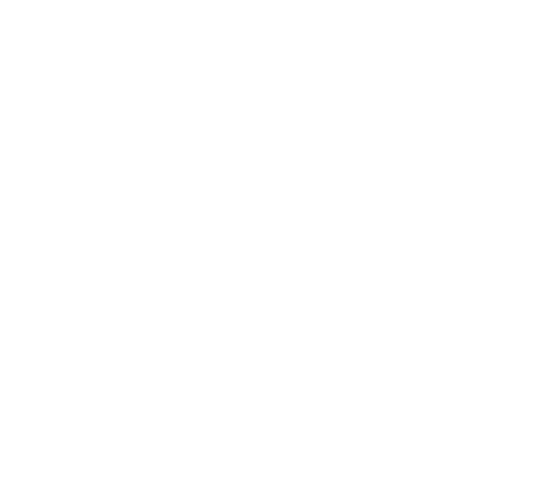
\includegraphics[width=0.5\textwidth,height=0.5\textheight,keepaspectratio]{pencil}
        \end{figure}
        \huge Mãos à obra

        \normalsize Primeiro programa simples em Assembly
    \end{center}
\end{frame}

\subsection{Primeiro programa}
\begin{frame}[fragile]{Exemplo de código}
    O código abaixo troca o \textit{Display-Mode} para 3 e pinta o pixel
    nas coordenadas (0, 0) de Amarelo-escuro (BGR 0, 15, 15):

    \begin{minted}[escapeinside=||]{asm}
main:
    ldr r0, |=0x04000000|
    ldr r1, |=0x403|
    strh r1, [r0]
    ldr r0, |=0x6000000|
    ldr r1, |=0x1EF|
    strh r1, [r0]
    \end{minted}

    Iremos supor que o código está salvo em um arquivo chamado
    \texttt{asm\_example.s}.
\end{frame}

\subsection{Compilação}

\begin{frame}{\subsecname}
    Como estamos em uma arquitetura diferente, precisamos de uma ferramenta
    (mais especificamente, uma \emph{Toolchain}) para o compilador que
    saiba o esquema de memória adequado. Para GBA, a ferramenta que
    utilizaremos é \emph{DevKitPro} e seu submódulo \emph{DevKitARM}.
\end{frame}

\begin{frame}[fragile]{\subsecname - Gerar o arquivo do jogo}
    \begin{enumerate}
        \item Compilar e gerar um arquivo-objeto:
        {\
            \tiny
            \begin{minted}{bash}
arm-none-eabi-as -mthumb -mthumb-interwork -c asm_example.s
            \end{minted}
        }

        \vspace{1em}
        \item Gerar um arquivo \texttt{.elf} (Executable and Linkable File):
        {\
            \tiny
            \begin{minted}{bash}
arm-none-eabi-as -mthumb -mthumb-interwork -specs=gba.specs asm_example.o -o asm_example.elf
            \end{minted}
        }

        \vspace{1em}
        \item Tradução/Limpeza para um executável puro:
        {\
            \tiny
            \begin{minted}{bash}
arm-none-eabi-objcopy -O binary asm_example.elf asm_example.gba
            \end{minted}

            OBS: a etapa acima é necessária apenas para limpar os símbolos
            de debug que vêm no \texttt{.elf}.
        }

        \vspace{1em}
        \item Consertar Header:
        {\
            \tiny
            \begin{minted}{bash}
gbafix asm_example.gba
            \end{minted}

            Todo jogo de GBA possui um Header que checka se o binário é um GBA
            válido. O \texttt{gbafix} trata de ajeitar o header para que seja
            válido.
        }
    \end{enumerate}
\end{frame}

\begin{frame}{Testando o jogo}
    \begin{figure}[H]
        \centering
        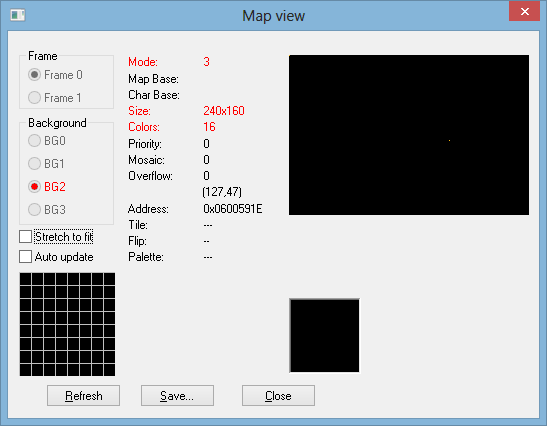
\includegraphics[width=1\textwidth,height=0.5\textheight,keepaspectratio]{mapview_asm_example}
    \end{figure}
\end{frame}
\begin{frame}[fragile]{\secname: Exemplo de execução de instrução}
    \vspace{-2em}
    \begin{minted}[escapeinside=||]{cpp-objdump}
|mov r0, \#0x04000000 ; r0 $\leftarrow$ 0x4000000|
|ldr r1, =\#0x403     ; r1 $\leftarrow$ 0x403|
|strh r1, [r0]       ; memory[r0] $\leftarrow$ r1|
    \end{minted}

    \vspace{-0.5em}
    \begin{tikzpicture}
        \draw (0, 0) rectangle (4, 4) node[midway, above=1.5cm] {Processador};
        \scriptsize\node at (2, 1.75) [align=right] {
            \begin{tabular}{|l|l|}
                \hline
                \texttt{r0} & \texttt{0x00000000} \\
                \texttt{r1} & \texttt{0x00000000} \\
                \texttt{r2} & \texttt{0x00000000} \\
                \texttt{r3} & \texttt{0x00000000} \\
                \texttt{r4} & \texttt{0x00000000} \\
                \texttt{r5} & \texttt{0x00000000} \\
                \ldots & \ldots \\
                \texttt{r15} & \texttt{0x08000004} \\\hline
            \end{tabular}
        };
        \foreach \x in {0,...,15} {
            \pgfmathsetmacro{\y}{(4 / 18)*(\x + 1)}
            \draw (4, \y) -- (6, \y);
        }

        \draw (6, 4.5) rectangle(10, 4) node[pos=.5] {Memória};
        \scriptsize\draw (6, 0) rectangle(10, 4) node[at start, above right, align=left] {
            \begin{tabular}{l|l}
                \texttt{0x00000000} & \texttt{0x0000} \\
                \texttt{0x00000002} & \texttt{0x0000} \\
                \ldots & \ldots \\
                \texttt{0x03000000} & \texttt{0xA011}\\
                \texttt{0x03000002} & \texttt{0x00FF}\\
                \texttt{0x03000004} & \texttt{0x09B0}\\
                \ldots & \ldots \\
                \texttt{0x04000000} & \texttt{0x0000}\\
                \ldots & \ldots \\
                \texttt{0x01FFFFFF} & \texttt{0x0000}
            \end{tabular}
        };
    \end{tikzpicture}
\end{frame}

\begin{frame}[fragile]{\secname: Exemplo de execução de instrução}
    \vspace{-2em}
    \begin{minted}[escapeinside=||]{cpp-objdump}
|\color{red}mov r0, \#0x04000000 ; r0 $\leftarrow$ 0x4000000|
|ldr r1, =\#0x403     ; r1 $\leftarrow$ 0x403|
|strh r1, [r0]       ; memory[r0] $\leftarrow$ r1|
    \end{minted}

    \vspace{-0.5em}
    \begin{tikzpicture}
        \draw (0, 0) rectangle (4, 4) node[midway, above=1.5cm] {Processador};
        \scriptsize\node at (2, 1.75) [align=right] {
            \begin{tabular}{|l|l|}
                \hline
                \texttt{r0} & \texttt{0x04000000} \\
                \texttt{r1} & \texttt{0x00000000} \\
                \texttt{r2} & \texttt{0x00000000} \\
                \texttt{r3} & \texttt{0x00000000} \\
                \texttt{r4} & \texttt{0x00000000} \\
                \texttt{r5} & \texttt{0x00000000} \\
                \ldots & \ldots \\
                \texttt{r15} & \texttt{0x08000004} \\\hline
            \end{tabular}
        };
        \foreach \x in {0,...,15} {
            \pgfmathsetmacro{\y}{(4 / 18)*(\x + 1)}
            \draw (4, \y) -- (6, \y);
        }

        \draw (6, 4.5) rectangle(10, 4) node[pos=.5] {Memória};
        \scriptsize\draw (6, 0) rectangle(10, 4) node[at start, above right, align=left] {
            \begin{tabular}{l|l}
                \texttt{0x00000000} & \texttt{0x0000} \\
                \texttt{0x00000002} & \texttt{0x0000} \\
                \ldots & \ldots \\
                \texttt{0x03000000} & \texttt{0xA011}\\
                \texttt{0x03000002} & \texttt{0x00FF}\\
                \texttt{0x03000004} & \texttt{0x09B0}\\
                \ldots & \ldots \\
                \texttt{0x04000000} & \texttt{0x0000}\\
                \ldots & \ldots \\
                \texttt{0x01FFFFFF} & \texttt{0x0000}
            \end{tabular}
        };
    \end{tikzpicture}
\end{frame}

\begin{frame}[fragile]{\secname: Exemplo de execução de instrução}
    \vspace{-2em}
    \begin{minted}[escapeinside=||]{cpp-objdump}
|mov r0, \#0x04000000 ; r0 $\leftarrow$ 0x4000000|
|\color{red}ldr r1, =\#0x403     ; r1 $\leftarrow$ 0x403|
|strh r1, [r0]       ; memory[r0] $\leftarrow$ r1|
    \end{minted}

    \vspace{-0.5em}
    \begin{tikzpicture}
        \draw (0, 0) rectangle (4, 4) node[midway, above=1.5cm] {Processador};
        \scriptsize\node at (2, 1.75) [align=right] {
            \begin{tabular}{|l|l|}
                \hline
                \texttt{r0} & \texttt{0x04000000} \\
                \texttt{r1} & \texttt{0x00000403} \\
                \texttt{r2} & \texttt{0x00000000} \\
                \texttt{r3} & \texttt{0x00000000} \\
                \texttt{r4} & \texttt{0x00000000} \\
                \texttt{r5} & \texttt{0x00000000} \\
                \ldots & \ldots \\
                \texttt{r15} & \texttt{0x08000006} \\\hline
            \end{tabular}
        };
        \foreach \x in {0,...,15} {
            \pgfmathsetmacro{\y}{(4 / 18)*(\x + 1)}
            \draw (4, \y) -- (6, \y);
        }

        \draw (6, 4.5) rectangle(10, 4) node[pos=.5] {Memória};
        \scriptsize\draw (6, 0) rectangle(10, 4) node[at start, above right, align=left] {
            \begin{tabular}{l|l}
                \texttt{0x00000000} & \texttt{0x0000} \\
                \texttt{0x00000002} & \texttt{0x0000} \\
                \ldots & \ldots \\
                \texttt{0x03000000} & \texttt{0xA011}\\
                \texttt{0x03000002} & \texttt{0x00FF}\\
                \texttt{0x03000004} & \texttt{0x09B0}\\
                \ldots & \ldots \\
                \texttt{0x04000000} & \texttt{0x0000}\\
                \ldots & \ldots \\
                \texttt{0x01FFFFFF} & \texttt{0x0000}
            \end{tabular}
        };
    \end{tikzpicture}
\end{frame}

\begin{frame}[fragile]{\secname: Exemplo de execução de instrução}
    \vspace{-2em}
    \begin{minted}[escapeinside=||]{cpp-objdump}
|mov r0, \#0x04000000 ; r0 $\leftarrow$ 0x4000000|
|ldr r1, =\#0x403     ; r1 $\leftarrow$ 0x403|
|\color{red}strh r1, [r0]       ; memory[r0] $\leftarrow$ r1|
    \end{minted}

    \vspace{-0.5em}
    \begin{tikzpicture}
        \draw (0, 0) rectangle (4, 4) node[midway, above=1.5cm] {Processador};
        \scriptsize\node at (2, 1.75) [align=right] {
            \begin{tabular}{|l|l|}
                \hline
                \texttt{r0} & \texttt{0x04000000} \\
                \texttt{r1} & \texttt{0x00000403} \\
                \texttt{r2} & \texttt{0x00000000} \\
                \texttt{r3} & \texttt{0x00000000} \\
                \texttt{r4} & \texttt{0x00000000} \\
                \texttt{r5} & \texttt{0x00000000} \\
                \ldots & \ldots \\
                \texttt{r15} & \texttt{0x08000008} \\\hline
            \end{tabular}
        };
        \foreach \x in {0,...,15} {
            \pgfmathsetmacro{\y}{(4 / 18)*(\x + 1)}
            \draw (4, \y) -- (6, \y);
        }

        \draw (6, 4.5) rectangle(10, 4) node[pos=.5] {Memória};
        \scriptsize\draw (6, 0) rectangle(10, 4) node[at start, above right, align=left] {
            \begin{tabular}{l|l}
                \texttt{0x00000000} & \texttt{0x0000} \\
                \texttt{0x00000002} & \texttt{0x0000} \\
                \ldots & \ldots \\
                \texttt{0x03000000} & \texttt{0xA011}\\
                \texttt{0x03000002} & \texttt{0x00FF}\\
                \texttt{0x03000004} & \texttt{0x09B0}\\
                \ldots & \ldots \\
                \texttt{0x04000000} & \texttt{0x0403}\\
                \ldots & \ldots \\
                \texttt{0x01FFFFFF} & \texttt{0x0000}
            \end{tabular}
        };
    \end{tikzpicture}
\end{frame}


\section{Extras}

\begin{frame}{}
    \begin{center}
        \huge Extras
    \end{center}
\end{frame}

\subsection{DevKitPro}

\begin{frame}{\subsecname - Instalação}
    \begin{description}
        \item[Windows:]
            \begin{enumerate}
                \item Baixar a versão mais atualizada do DevKitProUpdater:
                    \url{http://sourceforge.net/projects/devkitpro/files/Automated\%20Installer/}
                \item Executar o instalador. É possível customizar a instalar
                    somente o DevKitARM e ainda retirar os exemplos, se
                    necessário.
            \end{enumerate}
        \item[Linux:]
            Seguir o guia:
            \url{https://docs.google.com/document/d/1ieTi_zARtRsm93u6QDUkRLEDU7JGlYOKGSNuII0d02s/pub}
    \end{description}
\end{frame}

\subsection{VisualBoyAdvance}

\begin{frame}{\subsecname}
    \begin{figure}
        \centering
        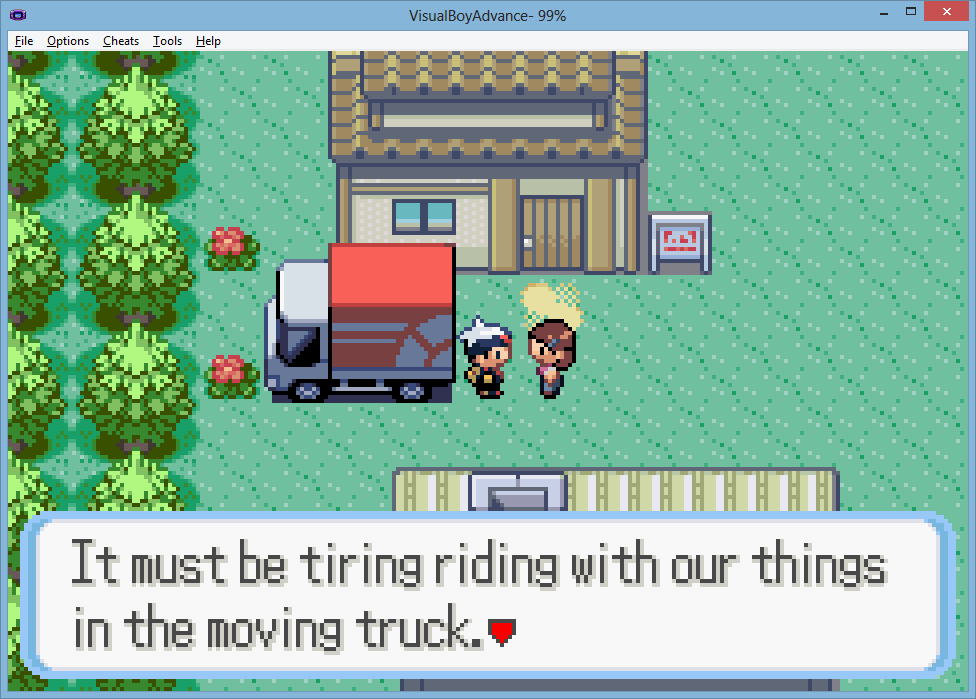
\includegraphics[width=1\textwidth,height=0.5\textheight,keepaspectratio]{game_example}
    \end{figure}
\end{frame}

\begin{frame}{\subsecname: Recursos}
    \begin{itemize}
        \item Emulação rápida;
        \item Leve e de fácil configuração;
        \item Ferramentas para desenvolvedor (não disponível na versão VBA-M):
            \begin{itemize}
                \item Disassemble;
                \item Logging;
                \item IO Viewer;
                \item Map Viewer;
                \item Palette Viewer;
                \item Memory Viewer;
                \item OAM Viewer;
                \item Tile Viewer;
                \item Habilitar/Desabilitar Layers.
            \end{itemize}
    \end{itemize}
\end{frame}

\begin{frame}{\subsecname: Disassemble}
    \begin{figure}
        \centering
        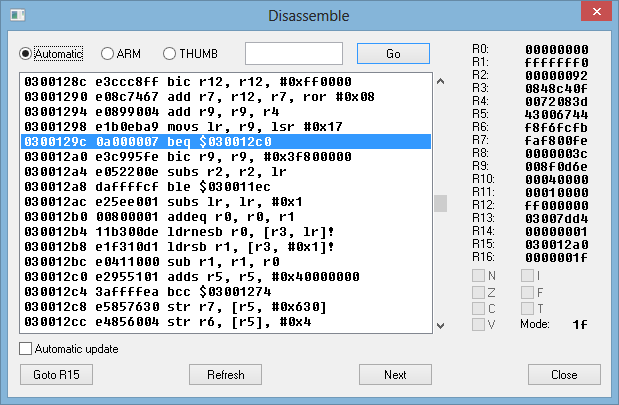
\includegraphics[width=1\textwidth,height=0.5\textheight,keepaspectratio]{disassemble}
    \end{figure}
\end{frame}

\begin{frame}{\subsecname: Logging}
    \begin{figure}
        \centering
        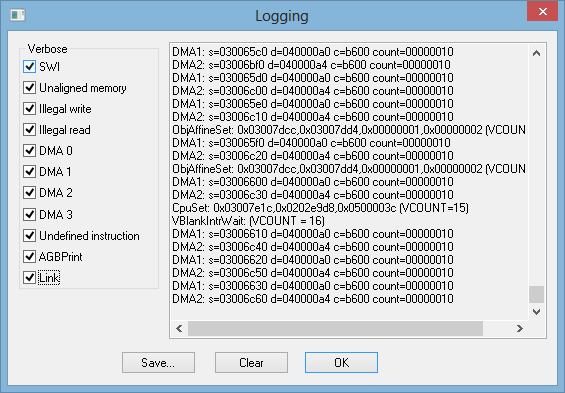
\includegraphics[width=1\textwidth,height=0.5\textheight,keepaspectratio]{loggingview}
    \end{figure}
\end{frame}

\begin{frame}{\subsecname: IO Viewer}
    \begin{figure}
        \centering
        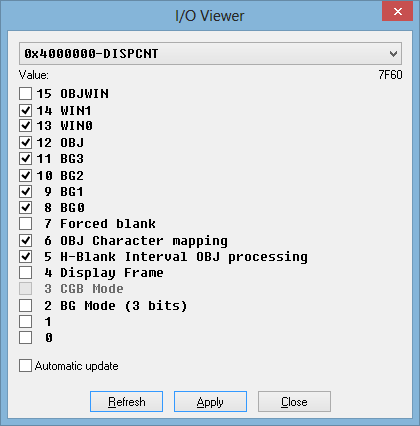
\includegraphics[width=1\textwidth,height=0.5\textheight,keepaspectratio]{ioview}
    \end{figure}
\end{frame}

\begin{frame}{\subsecname: Map Viewer}
    \begin{figure}
        \centering
        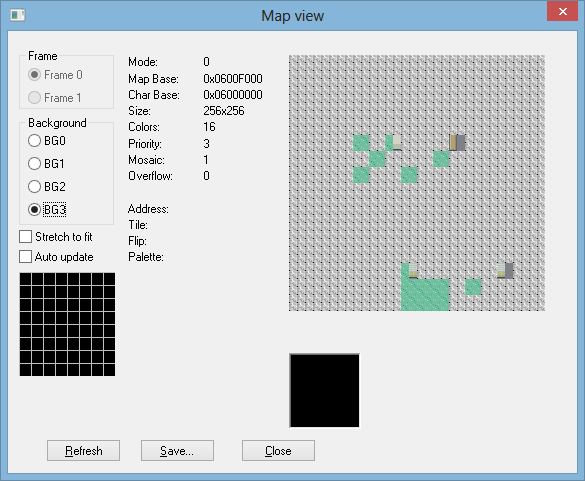
\includegraphics[width=1\textwidth,height=0.4\textheight,keepaspectratio]{mapview}
        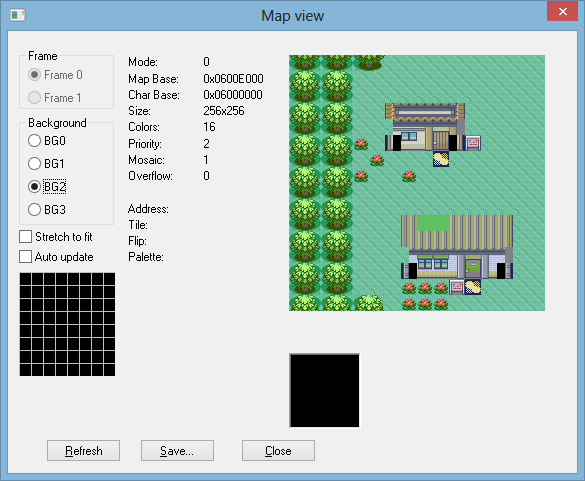
\includegraphics[width=1\textwidth,height=0.4\textheight,keepaspectratio]{mapview2}
    \end{figure}
    \vspace{-2.5em}
    \begin{figure}
        \centering
        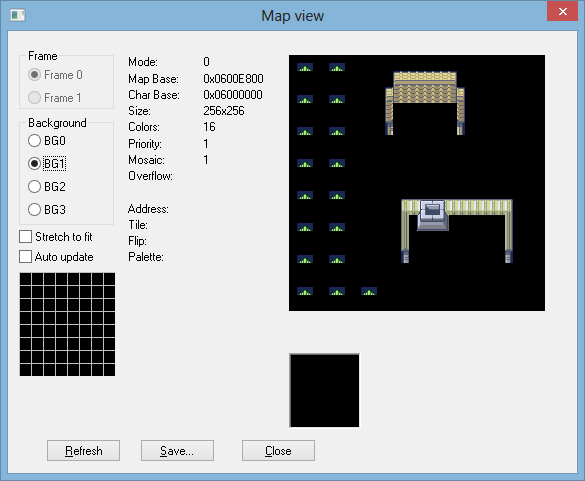
\includegraphics[width=1\textwidth,height=0.4\textheight,keepaspectratio]{mapview3}
        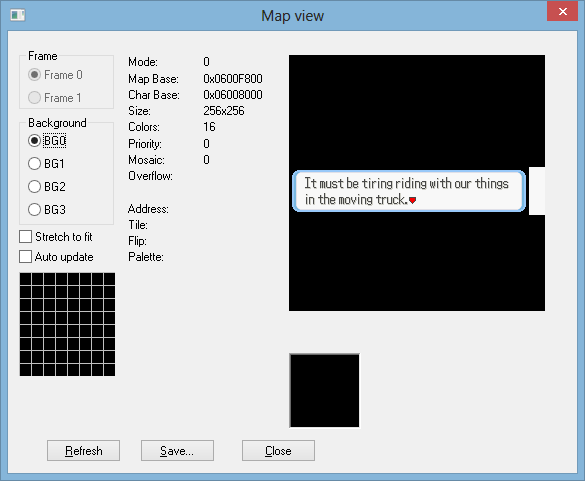
\includegraphics[width=1\textwidth,height=0.4\textheight,keepaspectratio]{mapview4}
    \end{figure}
\end{frame}

\begin{frame}{\subsecname: Memory Viewer}
    \begin{figure}
        \centering
        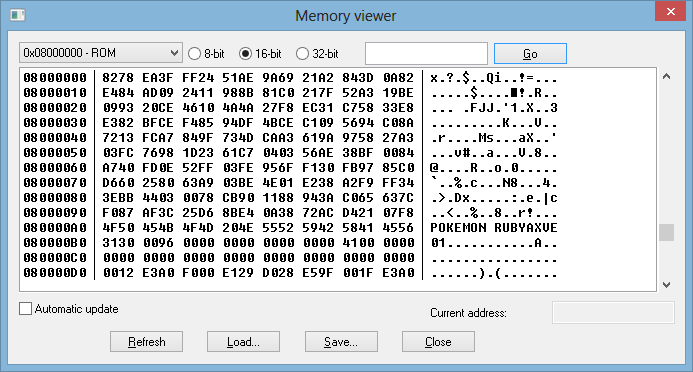
\includegraphics[width=1\textwidth,height=0.5\textheight,keepaspectratio]{memview}
    \end{figure}
\end{frame}

\begin{frame}{\subsecname: OAM Viewer}
    \begin{figure}
        \centering
        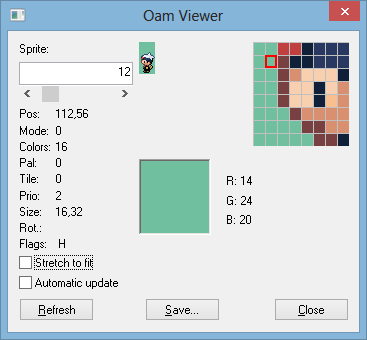
\includegraphics[width=1\textwidth,height=0.5\textheight,keepaspectratio]{oamview}
    \end{figure}
\end{frame}

\begin{frame}{\subsecname: Palette Viewer}
    \begin{figure}
        \centering
        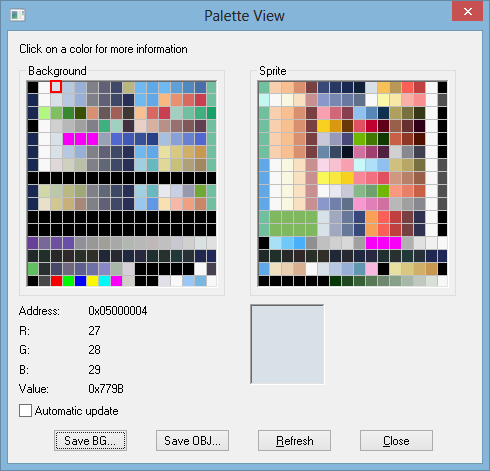
\includegraphics[width=1\textwidth,height=0.5\textheight,keepaspectratio]{paletteview}
    \end{figure}
\end{frame}

\begin{frame}{\subsecname: Tile Viewer}
    \begin{figure}
        \centering
        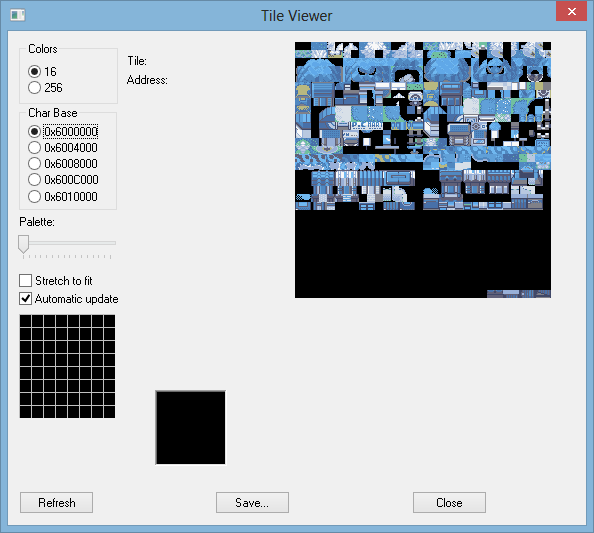
\includegraphics[width=1\textwidth,height=0.5\textheight,keepaspectratio]{tileview}
    \end{figure}
\end{frame}


\bibliographystyle{ieeetr}
\begin{frame}[allowframebreaks]{Referências/Bibliografia}
    \bibliography{class}
    \nocite{*}
\end{frame}

\begin{frame}{Obrigado!}
    \begin{center}
        \Huge Perguntas?
    \end{center}
\end{frame}

\end{darkframes}
\end{document}
